% \section{Modelo usando propiedades físico-químicas de la proteína}

En esta sección generamos un nuevo dataset buscando nuevas fuentes de información de carácter físico-químico de las proteínas. Estas variables provienen de dos fuentes principales:

\begin{itemize}
    \item El módulo ProtParam proveniente de la biblioteca Biopython \cite{Chapman:2000:BPT:360262.360268}
    \item La base de datos SNVBox del laboratorio Karchin \cite{Wong2011}
\end{itemize}

Para el análisis de estas variables usamos la tabla Humsavar. La tabla Humsavar (a Noviembre 2017) está compuesta originalmente por 75,769 variantes (o ``mutantes'') de las cuales 39,653 son benignas (52\%), 28,855 (38\%) están asociadas a enfermedades y 7,261 (10\%) no están clasificadas. Las variantes no clasificadas fueron descartadas. 

\section{Extracción de variables usando Biopython}

La primera fuente que utilizamos, por su relativa practicidad de uso en la extracción de un conjunto de variables físico-químicas de la proteína, fue el módulo ProtParam de la biblioteca Biopython. Esta biblioteca es un set de herramientas escritas en Python, desarrollada por un equipo internacional de desarrolladores para el área de la bioinformática, y posee una licencia de uso libre.
El nombre ProtParam proviene de \textit{Protein Parameters} (parámetros de la proteína) y está basado en la herramienta homónima del server proteómico Expasy. Para ser utilizado el módulo requiere el \textit{accession number} de la proteína (identificador único) o una subsecuencia de la misma, para poder acceder a los parámetros calculados, que son los siguientes:

\begin{itemize}
    \item Punto isoeléctrico teórico (ISO\_POINT): pH en el que la proteína (o subsecuencia) tiene carga nula. 
    \item Aromaticidad (AROM): La frecuencia relativa de la subsecuencia Phe+Trp+Tyr (Fenilalanina, Triptófano y Tirosina). 
    \item Índice de inestabilidad (INST): Testea la estabilidad de la subsecuencia. Cualquier valor superior a 40 indica inestabilidad, es decir una corta semivida.
    \item Flexibilidad (FLEX): Método de Flexibilidad implementado por Vihinen et Al.  
    \item Promedio de hidrofobicidad (GRAVY): La suma de valores de hidrofobicidad de cada uno de los aminoácidos que componen la subsecuencia de la proteína.
\end{itemize}

Para poder utilizar el módulo ProtParam recurrimos a Uniprot con el fin de conseguir el proteoma humano en formato FASTA. El formato FASTA fue desarrollado por David Lipman y William Pearson en 1985, y originalmente fue incluido en un programa del mismo nombre utilizado para el alineamiento múltiple de secuencias. Una archivo FASTA puede incluir diferentes secuencias, no necesariamente de aminoácidos, y cada una de estas secuencias posee una línea de descripción al comienzo que empieza con el símbolo $>$. Por ejemplo, así se ve la secuencia de la Ovoalbúmina, una proteína de la especie Gallus gallus (gallina), o en otras palabras, la principal proteína que encontramos en la clara de los huevos (figura \ref{code:fasta_code})

\begin{figure}
% \centering
    \begin{verbatim}
    	>P01013 GENE X PROTEIN (OVALBUMIN-RELATED)
    	QIKDLLVSSSTDLDTTLVLVNAIYFKGMWKTAFNAEDTREMPFHVTKQESKPVQMMCMNNSFNVATLPAE
    	KMKILELPFASGDLSMLVLLPDEVSDLERIEKTINFEKLTEWTNPNTMEKRRVKVYLPQMKIEEKYNLTS
    	VLMALGMTDLFIPSANLTGISSAESLKISQAVHGAFMELSEDGIEMAGSTGVIEDIKHSPESEQFRADHP
    	FLFLIKHNPTNTIVYFGRYWSP
    \end{verbatim}
% \includegraphics{}
\caption{Ejemplo de código Fasta. Este código representa la proteína albúmina, donde cada letra representa un aminoácido, por ejemplo, las primeras 5 letras representan Q (glutamina), I (isoleucina), K (lisina), D (ácido aspártico) y L (leucina).}
\label{code:fasta_code}

\end{figure}
\pagebreak

A partir del proteoma obtenido se extrajeron las secuencias correspondientes a las proteínas del dataset Humsavar, y para cada una de ellas se tomó una subsecuencia de la misma de largo 7, alrededor de la posición donde se produjo la variante (figura \ref{fig:sequence_window}). En caso de que la variante se haya producido en los primeros o los últimos lugares, se toman aminoácidos a derecha o a izquierda según corresponda para completar el largo de la ventana.

% \begin{figure}
% \begin{textopo}
%   \labelstyle{hl}{diamond}{Black}{Blue}{White}{}
%   \sequence{PQALPSV[LQIAMAFGLAIGTLVQALG]HV%
%   SGAH[([NNE,30]hl[box[Black,Blue]:Half loop[White]]=INPAVTVACL)]VGCHVSFLR}
%   \Nterm{extra} \hideNterm \hideCterm \hidelegend \labelTM{1}{II}
%   \labeloutside[right]{extra}
% \end{textopo}
% \caption{A `half loop' example}\label{fighalf}
% \end{figure}

\begin{figure}[H]
    \centering
    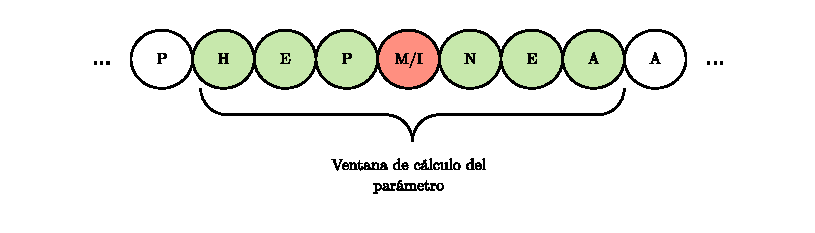
\includegraphics[scale=1.2]{documents/latex/figures/3/structural/protparam.pdf}
    \caption{Secuencia de aminoácidos de la proteína Arilacetamida deacetilasa (Q5VUY0). La ventana de la subsecuencia está marcada en verde, y la posición rojo es la mutación estudiada. En este caso la metionina (M) en la posición 307 fue reemplazada por una isoleucina (I).}
    \label{fig:sequence_window}
\end{figure}

A partir de los parámetros parámetros calculados en ProtParam, buscamos capturar la magnitud del cambio debido a la variante. Estos cambios pueden ser responsables de un efecto patogénico. Por ejemplo, si la región afectada por la variante pasa a ser hidrofílica en vez de hidrofóbica esta será más propensa a efectos adversos \cite{doi:10.1093/bioinformatics/btt308}.

En este sentido, generamos dos variables que buscan reflejar la diferencia generada por la variante. Las variables son las siguientes: 

\begin{itemize}
    \item Diferencia (DIFF) 
    $$|x - x_{var}|$$
    \item Cociente de logaritmos (LOG\_RATIO)
    $$\frac{\log{(x + 1)}}{\log{(x_{var} + 1)}}$$  
\end{itemize}

donde $x$ representa al parámetro original y $x_{var}$ es igual al parámetro de la variante.

\section{Extracción de variables usando SNVBox}

Además de la información obtenida vía ProtParam, recurrimos a una base de datos llamada SNVBox. Esta base de datos fue elaborada y es actualmente mantenida por el Karchin Lab de la Universidad Johns Hopkins. Se encuentra en su versión 3.0 y sigue en desarrollo. SNVBox posee alrededor de 90 variables consideradas relevantes para detectar el impacto biológico de un SNV (\textit{Single Nucleotide Variant}). Existen distintos criterios para definir un SNV y su diferencia de un SNP, pero en este trabajo los usaremos de forma indistinta. SNVBox posee datos físico-químicos de la proteína, a nivel de aminoácido y también a nivel de los sitios de la proteína donde se encuentra la variante. Otra característica destacable de esta fuente es que posee dichas variables para todos los codones del exoma humano.

\section{Generación del dataset Físico-Químico}

Luego del proceso del extracción de variables de Biopython y SNVBox, generamos un nuevo dataset cruzando sus atributos con las variantes de Humsavar. En el caso de los atributos relativos a los aminoácidos, pudimos cruzarlos usando la columna del dataset referente al identificador de la proteína, la posición de la variante, y el par de aminoácidos que se intercambiaron. Una vez agregadas todas las variantes a la tabla Humsavar, removimos todas aquellas variantes sin clasificación (etiqueta \textit{Unclassified}). El dataset resultante (denominado dataset Físico-Químico) está compuesto por 68,508 observaciones y 50 variables, incluyendo la variable de respuesta (o tipo), de las cuales 39,653 son benignas (no se encontraron reportes de enfermedades en la literatura), y 28,855 variantes están asociadas a alguna enfermedad. 

\section{Descripción estadística del dataset Físico-Químico}

Luego de la creación del dataset realizamos una exploración estadística del mismo, tal como hicimos en el dataset VarQ Curado. Calculamos la media (\textit{mean}), el desvío estándar (\textit{std}), el mínimo, el máximo y los cuartiles (25\%, 50\%, y 75\%). También calculamos el AUC univariado para cada una de las variables continuas del dataset. Con respecto al AUC univariado en las variables de Protparam (tabla \ref{tab:protparam_vars}), notamos que la versión DIFF de los parámetros es mejor (anti) predictor que sus versiones LOG\_RATIO en todos los casos.


\begin{table}[H]
\centering
\begin{tabular}{|l|l|l|l|l|l|l|l|l|}
\hline
Variable & mean & std & min & 25\% & 50\%  & 75\% & max & AUC \\ \hline
AROM\_DIFF  & 0.02  & 0.02  & 0.00 & 0.00 & 0.00  & 0.01 & 0.22  & 0.59 \\ \hline
AROM\_LOG\_RATIO & 1.97 & 0.33 & 1.00 & 1.94 & 1.94  & 1.94 & 3.66  & 0.53 \\ \hline
ISO\_POINT\_DIFF & 0.69  & 0.98 & 0.00  & 0.00 & 0.17  & 1.22 & 6.30  & 0.56 \\ \hline
ISO\_POINT\_LOG\_RATIO & 2.00 & 0.08 & 1.69 & 1.99 & 2.00  & 2.01 & 2.45  & 0.51 \\ \hline
GRAVY\_DIFF & 0.23 & 0.17 & 0.00 & 0.09 & 0.20  & 0.33 & 1.67  & 0.55 \\ \hline
GRAVY\_LOG\_RATIO & 2x10$^{12}$ & 1.2x$10^{14}$ & -3.3x10$^{15}$ & 1.43 & 1.94 & 2.43 & 9.6x10$^{15}$ & 0.48 \\\hline
INST\_DIFF & 14.02 & 13.27 & 0.00 & 4.20 & 10.09 & 20.10 & 139.00 & 0.49 \\ \hline
INST\_LOG\_RATIO & 2.06 & 2.27 & -84.77 & 1.96 & 2.01  & 2.09 & 453 & 0.48 \\ \hline
FLEX\_DIFF & 0.01 & 0.01 & 0.00 & 0.00 & 0.01  & 0.01  & 0.05 & 0.54 \\ \hline
FLEX\_LOG\_RATIO & 2.00 & 0.01 & 1.97 & 1.99 & 2.00  & 2.01  & 2.03 & 0.47 \\ \hline
\end{tabular}
\caption{Variables extraídas de Protparam}
\label{tab:protparam_vars}
\end{table}

% \newpage

Con respecto al AUC univariado de las variables extraídas de SNVBox, notamos que las mejores variables en este respecto son las aportadas por algunas de las matrices de sustitución (EX, PAM250 y BLOSUM). En este caso son buenos anti-predictores, lo que indica que un valor bajo en esta matrix aporta una mayor probabilidad de ser patogénica (tabla \ref{tab:snvbox_amino}). El mejor predictor en este set de variables es la valor en la matriz de distancias GRANTHAM.  



% \newpage

% \subsection{Variables extraídas de SNVBox relativas a sustitución de aminoácidos}

\begin{table}[H]
\centering
\begin{tabular}{|l|l|l|l|l|l|l|l|l|}
\hline
Variable & mean   & std    & min    & 25\%  & 50\%   & 75\% & max & AUC    \\ \hline
CHARGE            & 0.00  & 0.71   & -2.00  & 0.00  & 0.00   & 0.00 & 2.00 & 0.50   \\ \hline
VOLUME            & -0.16  & 1.70   & -5.59  & -1.40 & -0.16  & 0.96 & 5.59 & 0.48   \\ \hline
HYDROPHOBICITY    & -0.63  & 6.81   & -15.70 & -3.10 & -0.40  & 1.90 & 15.70 & 0.52  \\ \hline
GRANTHAM          & 79.96  & 48.06  & 5.00   & 43.00 & 74.00  & 102.00 & 215.00 &  \textbf{0.63} \\ \hline
POLARITY          & -0.25  & 2.72   & -8.10  & -2.20 & -0.10  & 1.10   & 8.10 & 0.52   \\ \hline
EX                & 28.99  & 10.95  & -1.00  & 21.00 & 29.00  & 35.00  & 61.00 & \textbf{0.35}  \\ \hline
PAM250            & 0.16   & 1.68   & -5.40  & -1.00 & 0.20   & 1.40   & 5.30 & \textbf{0.36}   \\ \hline
BLOSUM            & -0.58  & 1.65   & -4.00  & -2.00 & -1.00  & 1.00   & 3.00 & \textbf{0.35}   \\ \hline
JM                & 0.80   & 1.24   & -1.73  & -0.50 & 1.05   & 1.66   & 3.22 & 0.40   \\ \hline
VB                & 19.78  & 14.64  & 0.00   & 8.00  & 17.00  & 29.00  & 55.00 & 0.42  \\ \hline
TRANSITION        & 0.00   & 0.00   & 0.00   & 0.00  & 0.00   & 0.00   & 0.01 & 0.47   \\ \hline
\end{tabular}
\caption{Variables extraídas de SNVBox relativas a sustitución de aminoácidos.}
\label{tab:snvbox_amino}

\end{table}

Las variables continuas poseen una cobertura para el 100\% del dataset exceptuando algunas variables calculadas por ProtParam por alcanzar valores extremos (las cuatro variables LOG\_RATIO), en los que se decidió reemplazar por nulos. En la figura \ref{fig:proporcion_nulos_structural} presentamos la proporción de nulos en dichas variables.

\begin{figure}[H]
    \centering
    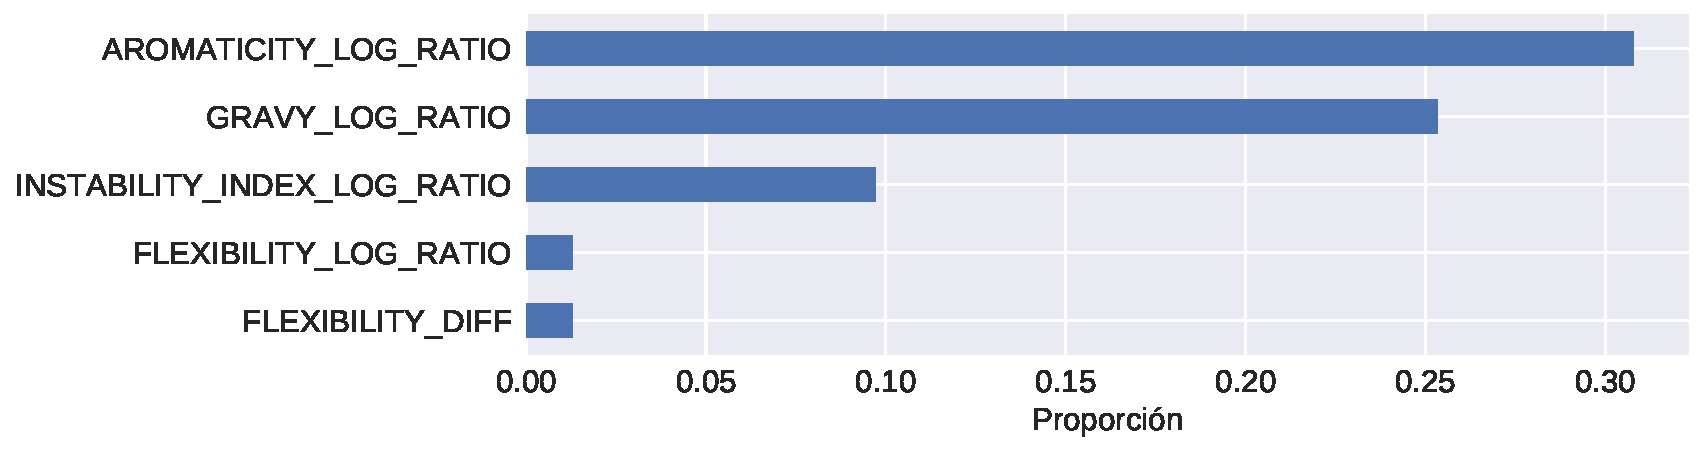
\includegraphics[scale=0.5]{documents/latex/figures/3/structural/proporcion_nulos_structural.pdf}
    \caption{Variables continuas con menor cobertura.}
    \label{fig:proporcion_nulos_structural}
\end{figure}

Describimos 21 variables de nuestro dataset. Las 29 variables restantes son extraídas de SNVBox relativas a proteínas y son todas categóricas de tipo \textit{Boolean} por lo que destacamos algunos datos de relevancia (ver apéndice para un listado completo). 


Todas estas variables tienen una cobertura para aproximadamente el 31.5\% de las variantes del dataset, y cada una de ellas poseen valor Falso para un porcentaje superior al 90\% de las variantes de la tabla, exceptuando las variables \textbf{TRANSMEM} (82\%), \textbf{REP} (87\%), \textbf{REGIONS} (70\%) y \textbf{PPI} (87\%). 

El \textit{Balanced Accuracy} de estas variables oscilan entre el 0.45 y 0.48, lo que connota un bajo poder predictivo univariado.

\newpage
% \subsection{Correlación entre las variables}

\begin{figure}[H]
    \centering
    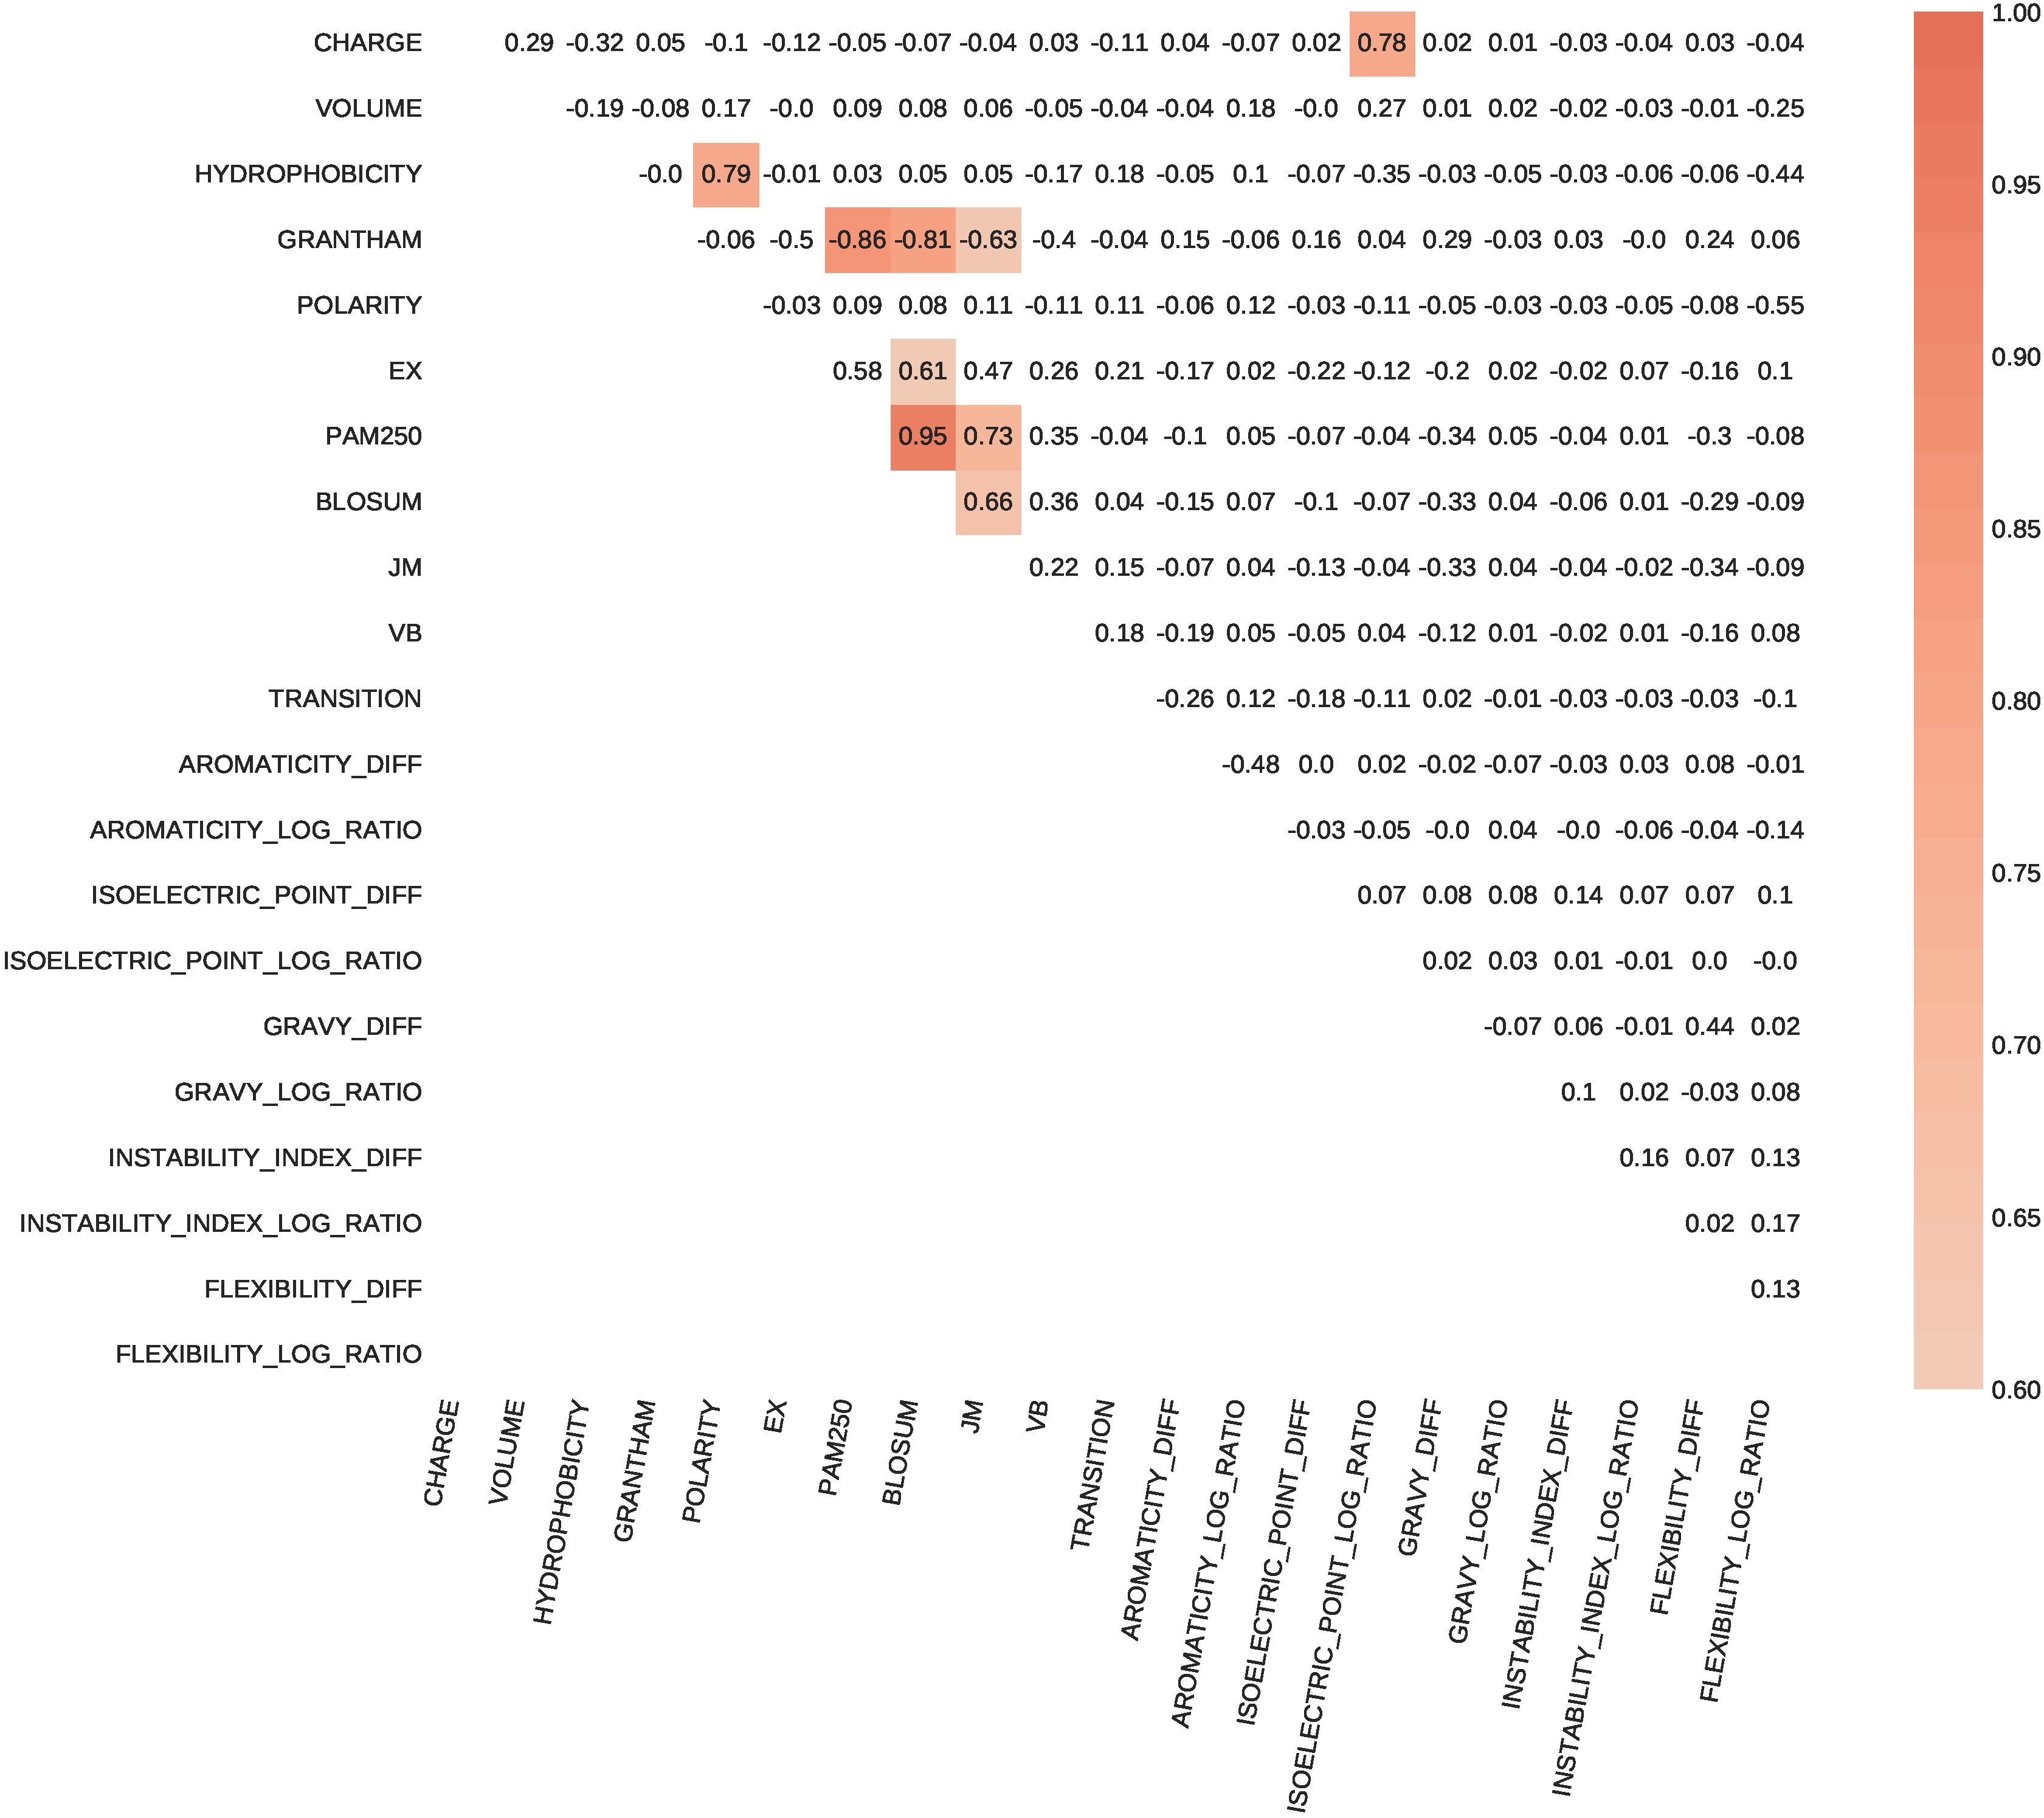
\includegraphics[scale=0.25]{documents/latex/figures/3/structural/structural_corr.pdf}
    \caption{Correlación de Spearman para las variables continuas del dataset Físico-Químico.}
    \label{fig:corrplot_structural}
\end{figure}

Por último, deseamos analizar la correlación entre las variables. Para esto usamos la correlación de Spearman dado que nos permite identificar correlaciones monotónicas. En la figura \ref{fig:corrplot_structural} podemos apreciar un cluster principal de variables altamente correlacionadas: Las matrices de sustitución (GRANTHAM, BLOSUM, JM, y EX). Por otro lado, encontramos a las variables POLARITY e HYDROPHOBICITY correlacionadas entre sí (0.79), como también a las variables CHARGE e ISOELECTRIC\_POINT\_LOG\_RATIO (0.78). Para este análisis decidimos excluir a las variables categóricas por tratarse de variables de tipo binarias con baja cobertura. 


% \subsection{Análisis de reducción de dimensionalidad}

% Una de las formas que nos permite ver que tan bien las variables de este dataset están separando nuestros tipos de SNPs, es usar reducción de dimensionalidad. El primer método que probamos fue el análisis de componentes principales (PCA), con el que generamos dos componentes, que son combinaciones lineales de nuestras variables iniciales de forma de maximizar la varianza, es decir el par de componentes que mejor explican la información completa.


% \newpage


\section{Generación del modelo}

Con este dataset generamos un modelo basado en un predictor Random Forest. 
Se eligió inicialmente este tipo de predictor por ser el que obtuvo los mejores resultados en el dataset VarQ Curado con respecto a otros predictores (SVMs y Regresión Logística). Otras de las ventajas que aporta este modelo es su facilidad para explicar la importancia de las variables y su relativa baja complejidad computacional, aunque es necesario que tener cuidado a este respecto con las correlaciones presentes entre las variables.

Para generar el modelo volvimos a construir un \textit{pipeline} muy similar al de la sección anterior, que consta de las siguientes etapas:

\begin{itemize}
 
\item \textbf{Imputación}: Las variables, cuyos valores eran nulos, se imputaron usando la mediana en el caso de las variables continuas, y con el valor más frecuente para las variables categóricas. 
\item \textbf{Escalado}: Las variables no fueron escaladas al no ser necesario en algoritmos de clasificacion basados en árboles de decisión, dado que se evalúan las variables de forma independiente. 
\item \textbf{Búsqueda de Hiperparámetros}: Para la búsqueda de hiperparámetros usamos \textit{Grid-Search} (búsqueda ``en cuadrícula'').
\end{itemize}


\section{Resultados del modelo Físico-Químico}

Como puede observarse en la figura \ref{fig:auc_structural}, a partir de este modelo se obtuvo un AUC de 0.72, que no supera lo obtenido por el modelo usando el dataset VarQ Curado. Las métricas observadas en la tabla \ref{structural_table} permiten dar cuenta de una precisión del 68\% con respecto a las observaciones patogénicas, es decir, el modelo está reportando un 32\% de variantes como patogénicas que no lo son (también conocido como error de tipo I), y un recall de 47\%, lo que indica que existe un 53\% de variantes patogénicas en nuestro dataset que no están siendo detectadas por nuestro modelo (error de tipo II). 

\begin{table}[H]
\centering
\begin{tabular}{|l|l|l|l|}
\hline
              & Precisión & Recall & F1-score \\ \hline
Benignas      & 0.68      & 0.81   & 0.74     \\ \hline
Patogénicas   & 0.65      & 0.47   & 0.54     \\ \hline
Promedio      & 0.66      & 0.67   & 0.66     \\ \hline
\end{tabular}
\caption{Métricas del modelo Random Forest aplicado al dataset Físico-Químico.}
\label{structural_table}
\end{table}


\section{Importancia de los atributos}

El algoritmo Random Forest nos permite identificar los mejores atributos en cada uno de los árboles del clasificador. En este caso, los primeros cuatro atributos refieren a matrices de sustitución (figura \ref{fig:importances_structural}). La quinta variable en importancia pertenece a ProtParam (AROMATICITY\_DIFF). 

También en la figura \ref{fig:importances_structural}, se observan variables con un nivel de importancia muy similar, como es el caso de PAM250, EX, BLOSUM y GRANTHAM. Todas estas variables corresponden a matrices de sustitutción, por lo que no es de extrañar que también exista un alto nivel de correlación entre ellas (ver figura \ref{fig:corrplot_structural}). 

Para analizar el impacto de clusters de variables altamente correlacionadas, usamos la herramienta \texttt{rfpimp} desarrollada por Terrence Parr y otros. Esta herramienta permite agrupar variables y analizar su importancia realizando permutaciones sobre las variables escogidas y reportando la perdida de precisión en el modelo. En la figura \ref{fig:importances_structural_cluster} vemos como las variables de hidrofobicidad y polaridad se ubican a la par de la matriz GRANTHAM. También aparecen nuevas variables en nivel de importancia, como DNA\_BIND y TRANSMEM (Sitio de unión de la proteína y region transmembrana respectivamente).


\pagebreak

\begin{figure}[H]
\centering
\begin{subfigure}[b]{0.7\textwidth}
    \centering
    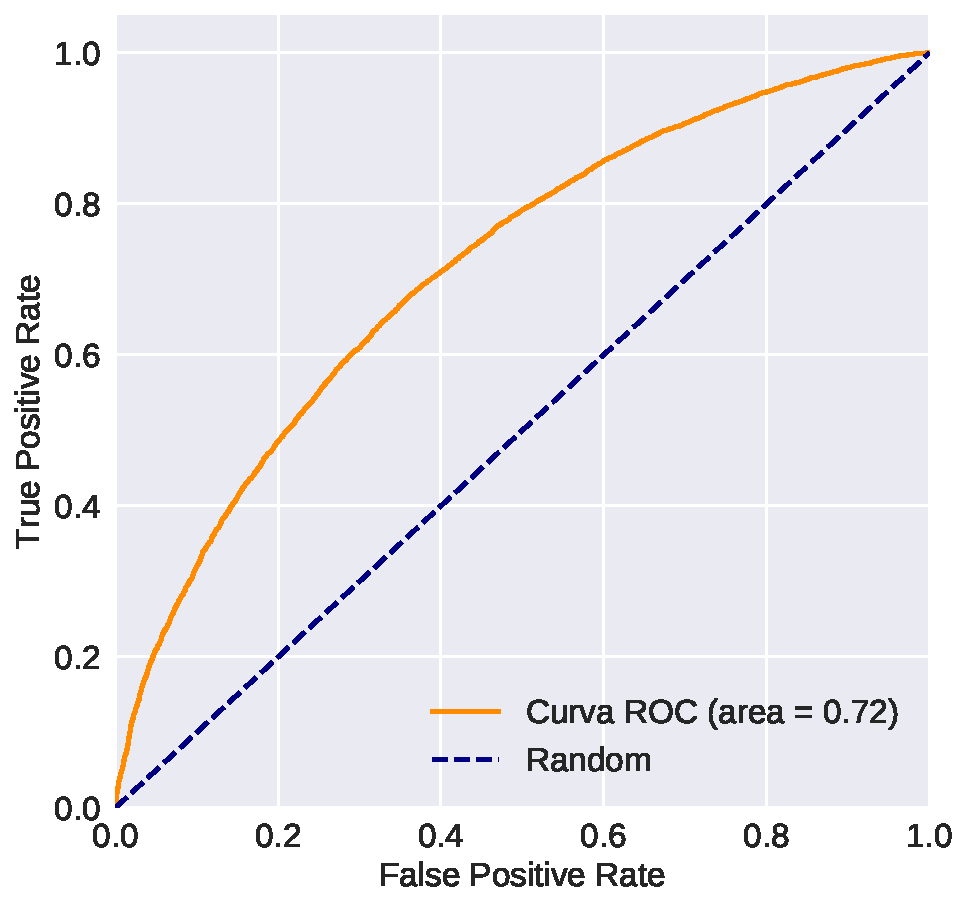
\includegraphics[width=\textwidth]{documents/latex/figures/3/structural/auc_structural.pdf}
    \caption{Curva AUC del algoritmo Random Forest aplicado al dataset Físico-Químico. La línea punteada corresponde a un predictor Random.}
    \label{fig:auc_structural}
\end{subfigure}

\hfill
\hfill

\begin{subfigure}[b]{0.7\textwidth}
    \centering
    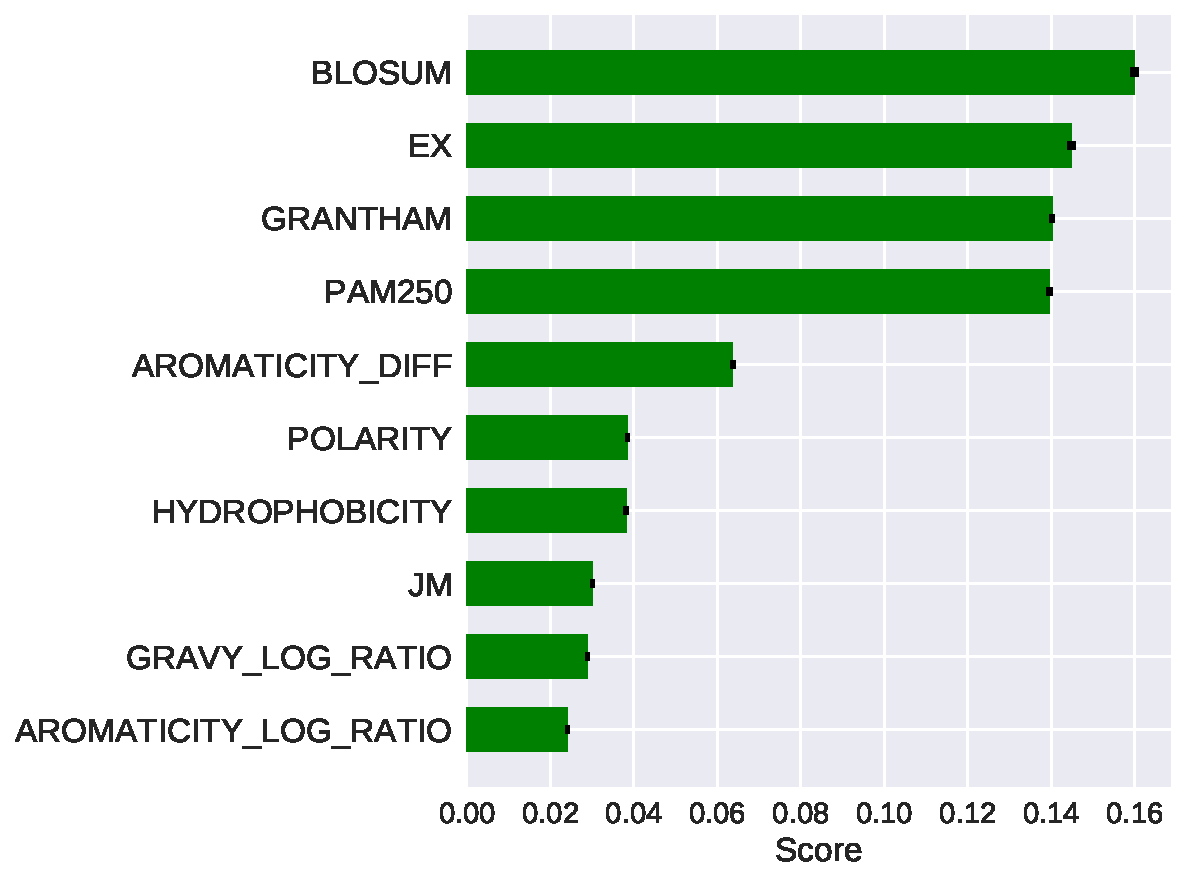
\includegraphics[width=\textwidth]{documents/latex/figures/3/structural/importances_structural.pdf}
    \caption{Los 10 atributos más importantes del modelo Random Forest usando el dataset Físico-Químico.}
    \label{fig:importances_structural}
\end{subfigure}

\caption{Curva AUC y atributos más importantes del modelo Físico-Químico}
\end{figure}

\newpage

\begin{figure}[H]
    \centering
    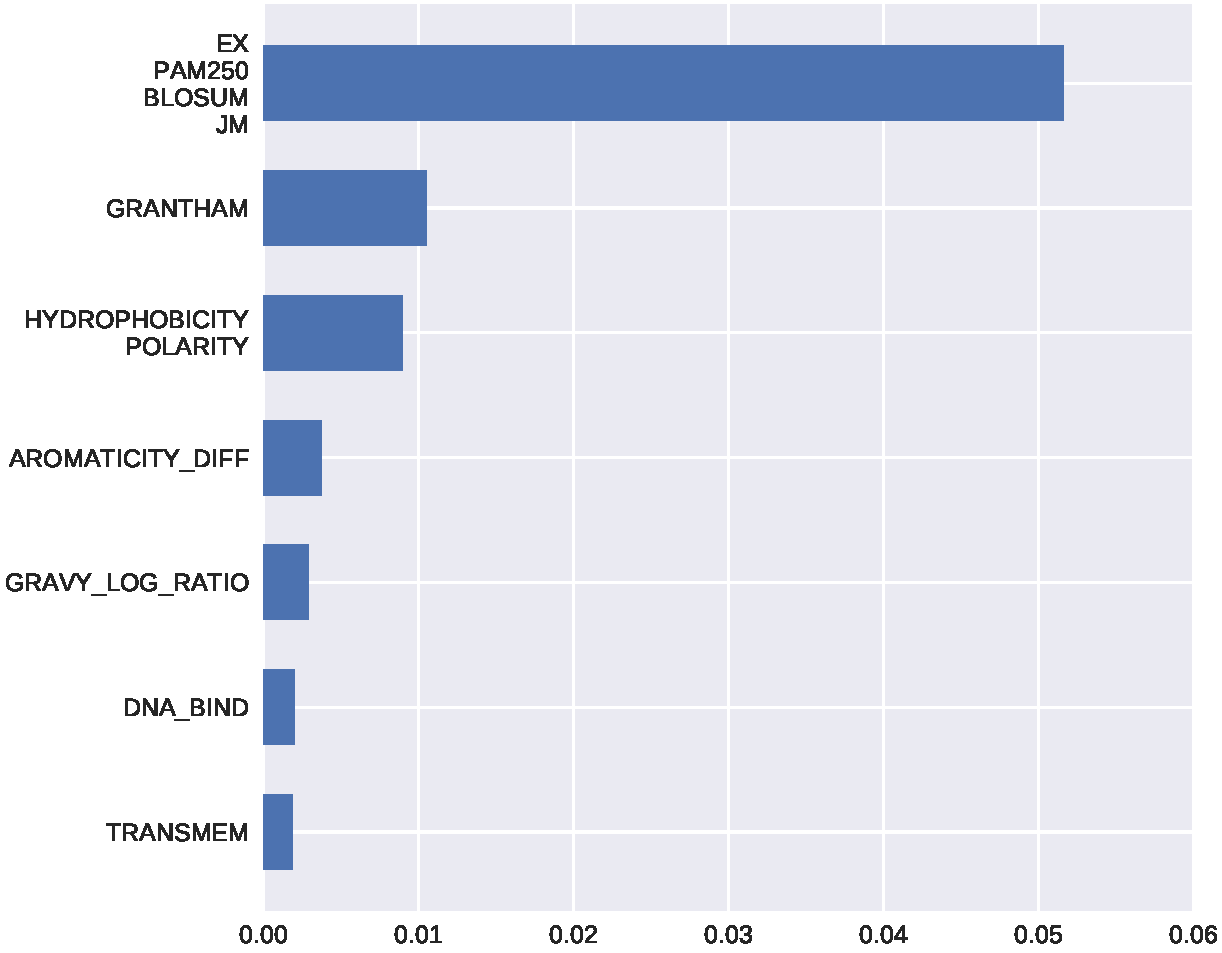
\includegraphics[scale=0.6]{documents/latex/figures/3/structural/structural_importance_cluster.pdf}
    \caption{Variación en la precisión al permutar clusters de variables correlacionadas ($>$ 0.90) del dataset Físico-Químico.}
    \label{fig:importances_structural_cluster}
\end{figure}

